\documentclass[tikz,border=2pt]{standalone}
\usepackage{amsmath}
\usetikzlibrary{arrows.meta}
\begin{document}
% Finite calling population, N=3 machines, c=1 mechanic, lambda=1, mu=3:
% up-rates lambda(n)=lambda(N-n)=3,2,1, down-rate mu(n)=mu=3,
% level crossing gives p=(9,9,6,2)/26.
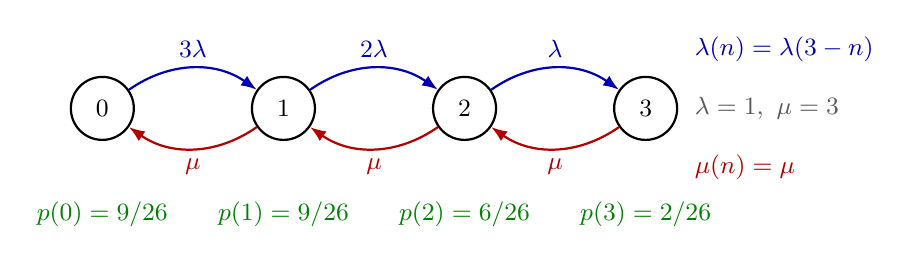
\begin{tikzpicture}[font=\small, >={Latex[length=2mm]},
  st/.style={circle, draw, thick, minimum size=8mm, inner sep=0pt}]
  \foreach \n in {0,1,2,3} {
    \node[st] (s\n) at (2.3*\n,0) {$\n$};
  }
  \foreach \a/\b/\r in {0/1/3\lambda, 1/2/2\lambda, 2/3/\lambda} {
    \draw[->, thick, blue!70!black] (s\a) to[bend left=35] node[above] {$\r$} (s\b);
    \draw[->, thick, red!70!black] (s\b) to[bend left=35] node[below] {$\mu$} (s\a);
  }
  \foreach \n/\p in {0/{9/26},1/{9/26},2/{6/26},3/{2/26}} {
    \node[green!50!black] at (2.3*\n,-1.35) {$p(\n)=\p$};
  }
  \node[blue!70!black, anchor=west] at (7.4,0.75) {$\lambda(n)=\lambda(3-n)$};
  \node[red!70!black, anchor=west] at (7.4,-0.75) {$\mu(n)=\mu$};
  \node[gray!70!black, anchor=west] at (7.4,0) {$\lambda=1,\ \mu=3$};
\end{tikzpicture}
\end{document}
